% ---------------------------------------------------------
% Project: PhD KAPPA
% File: materials.epi.tex
% Author: Andrea Discacciati
%
% Purpose: PCa epidemiology in COSM and Sweden (materials)
% ---------------------------------------------------------

\section{Description of COSM data and comparison with Swedish national data}
\label{sec:materialsepi}

In this section we will describe prostate cancer incidence and mortality in the COSM and will compare the results with Swedish national data. 

\subsection{Prostate cancer incidence}
\label{section:materials_incpca}

\subsubsection{Prostate cancer incidence in the COSM}
 
To date, the most recent available data at the Unit of Nutritional Epidemiology (Institute of Environmental Medicine, Karolinksa Institutet) include information on incident prostate cancer cases from 1 January 1998 until 31 December 2012 (SCR data). Data regarding tumor stage, Gleason score, and PSA levels are available until 31 December 2011 (NPCR data).

During 15 years of follow up (1998--2012), a total of 4,213 newly diagnosed cases were identified. Figure \ref{fig:ir_cosm} illustrates prostate cancer IRs by attained age and calendar year in the COSM. In particular, the solid lines are the predicted IRs from a single `flexible' PH model, where attained age was modeled using Restricted Cubic Splines (RCS) with 3 knots placed at the 10th, 50th, and 90th percentiles of the distribution of uncensored times (corresponding to 61, 72, and 82 years of age) \citep{harrell_regression_2001}. Moreover, the age-incidence curves were allowed to vary their shape across calendar year --- that is, the IRs between calendar years were not forced to be proportional. The hollow circles represent the observed IRs by 5-year categories of attained age (45--49, 50--54, \ldots, 80--84, and 85+) and calendar year (1998,\ldots,2012). Their size is proportional to the precision (inverse of the variance, assuming a Poisson distribution) of the estimate. As expected, the IRs increased steeply after 55--60 years of age, peaked around the age of 75 years, and generally declined thereafter. 

As noted in section \ref{section:descriptiveepidemiology}, prostate cancer incidence shows large geographical variation even within Sweden \citep{stattin_geographical_2005, jonsson_uptake_2011}. This could be partly due --- despite a uniform, equal-access health-care system --- to between-county differences in PSA-screening uptake  \citep{jonsson_uptake_2011}. Interestingly, the COSM study recruited participants from one high-incidence county (Västmanland) and one low-incidence county (Örebro) \citep{stattin_prostate_2014}. Not surprisingly, the age-adjusted prostate cancer IR was observed to be 16\% higher among those men residing in Västmanland county at the time of enrollment as compared with those residing in Örebro county, marginally over the 15 years of follow-up  [IRR: 1.16 (95\% CI: 1.09--1.23)]. Figure \ref{fig:appendix_ir_cosm} in the appendix shows the model-based predicted IRs by attained age, calendar year, and county of enrollment. The ratio between directly age-standardized IRs for Västmanland versus Örebro county was observed to be around 1.21 during the period 2000--2001, based on registry data \citep[table I]{stattin_geographical_2005}. %There was however evidence of effect modification by calendar year (Likelihood Ratio (LR) test: $\chi^2=53.6$, df = 14, $p \le 0.001$), with IRRs ranging from 0.91 (95\% CI: 0.74--1.12) for 2005, to 1.95 (95\% CI: 1.52--2.50) for 2011. 

\begin{sidewaysfigure}
\centering
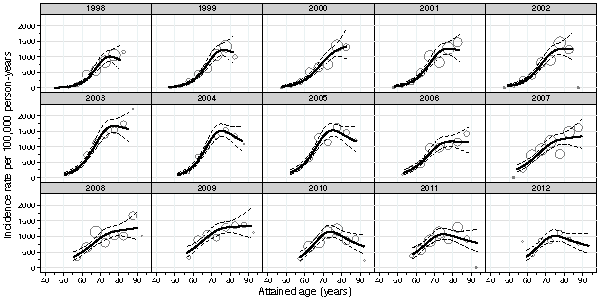
\includegraphics[width=\linewidth]{figures/ir_cosm.pdf}
\caption[Incidence rate of prostate cancer in the COSM by calendar year and attained age]{Incidence rate of prostate cancer in the COSM, conditional on calendar year and attained age. The solid line is the model-based predicted incidence rate, while dashed lines are 95\% confidence intervals. The hollow circles represent the observed incidence rate by calendar year and 5-year groups of attained age. Their size is proportional to the precision (inverse of the variance) of the estimate.}
\label{fig:ir_cosm}
\end{sidewaysfigure}

\subsubsection{Comparison with Swedish national data}
To the best of my knowledge, the only comparison between COSM and Swedish data in terms of prostate cancer incidence was carried out by  \citet[section~5.4]{orsini_physical_2008} in his PhD thesis. That analysis, which showed a remarkable good agreement between COSM and Swedish national data, was however limited to year 1998 only.

Information about the number of incident prostate cancer cases  by 5-year classes of age ($a=1,\ldots,9=$ ``45--49'',\dots,``85+'') and calendar year ($c=1998,\ldots,2012$) was available from the NBHW website ($d_{a,c}$),\footnote{\href{http://www.socialstyrelsen.se/statistik/statistikdatabas/cancer/}{\texttt{http://www.socialstyrelsen.se/statistik/statistikdatabas/cancer/}}} while the total number of men for the same categories  was available from the SCB website ($N_{a,c}$).\footnote{\href{http://www.scb.se/sv\_/Hitta-statistik/Statistik-efter-amne/Befolkning/}{\texttt{http://www.scb.se/sv\_/Hitta-statistik/Statistik-efter-amne/Befolkning/}}}  Under the assumption of constant prostate cancer incidence within age and calendar-year categories, the corresponding IRs in the Swedish male population were calculated as
\begin{equation*}
h_{a,c}^* = -\log \left(1 - \frac{d_{a,c}}{N_{a,c}-\frac{d_{a,c}}{2}} \right).
\end{equation*}

Standardized Incidence Ratios (SIRs) were obtained comparing the observed number of incident prostate cancer cases in the COSM with the expected number of cases obtained by applying Swedish national rates to the COSM age and calendar-year structure \citep[section~2.3]{breslow_statistical_1987}.  The overall SIR was calculated as follows:
\begin{equation*}
\SIR_{\LargerCdot, \LargerCdot} = \frac{\sum\limits^{9}_{a=1}\sum\limits_{c=1998}^{2012}o_{a,c}}{\sum\limits_{a=1}^{9}\sum\limits_{c=1998}^{2012}h_{a,c}^* t_{a,c}} = \frac{\sum\limits^{9}_{a=1}\sum\limits_{c=1998}^{2012}o_{a,c}}{\sum\limits_{a=1}^{9}\sum\limits_{c=1998}^{2012}e_{a,c}},
\end{equation*}
where $o_{a,c}$ was the number of observed cases, $t_{a,c}$ the total person-years in the COSM, and $e_{a,c}$ the number of expected cases. Marginal SIRs over attained age or calendar year were calculated by summing over the appropriate index (which, following standard notation, is replaced by a dot). Lastly, SIRs conditional on both attained age and calendar year were calculated as $\mathrm{SIR}_{a,c} = o_{a,c}/e_{a,c}$, for a given combination of $a$ and $c$. %However, one must be aware that many of the cells contain only a small number of observed cases. 
Exact confidence intervals for the SIR can be calculated, under the assumption that the observed number of cases follows a Poisson distribution, using the formulae provided by \citet{ulm_simple_1990}, or directly from the Poisson p.d.f. by the Newton-Raphson method. Alternatively, the number of observed cases can be modeled as a flexible function of a number of covariates (in this case, calendar year and attained age). This can be done by means of, among different methods,  a multiplicative Poisson regression model --- that is, a Generalized Linear Model with logarithmic link and Poisson distribution for the outcome --- with an offset term containing the expected number of cases \citep{berry_analysis_1983, breslow_statistical_1987}.

Table \ref{table:appendix_sir_table} in the appendix reports the number of observed (top entry) and expected (bottom entry) prostate cancer cases according to attained age categories and calendar year in the COSM. Overall --- that is, marginally over categories of attained age and calendar year --- the $\SIR_{\LargerCdot,\LargerCdot}$ for prostate cancer was equal to $4213 / 3656 = 1.15$ (95\% exact CI: 1.12--1.19). 

Figure \ref{fig:sir} shows the observed SIRs (hollow circles) calculated marginally over categories of attained age (panel A), and over calendar year (panel B). Furthermore, in panel A, SIR was modeled as a function of calendar year using RCS with 4 knots at years 1999, 2003, 2007, and 2012 (solid line). Similarly, panel B exhibits SIR modeled as a function of attained age using RCS with 4 knots at ages 55, 65, 75 and 80 years (solid line). 

There was no evidence of an association between calendar year and SIR in the RCS model ($p_{\textrm{overall}}=0.21$) or in a simpler linear model ($p_{\textrm{linear}}=0.88$). Note how the SIR relative to 1998 was very close to 1 [$\SIR_{\LargerCdot,1998} = 168/173 = 1.03$ (95\% exact CI: 0.88--1.19), see table \ref{table:appendix_sir_table}], in line with what observed by \citet{orsini_physical_2008}. Conversely, attained age was observed to be associated with SIR in the RCS model ($p_{\textrm{overall}}<0.001$), with evidence of non-linearity ($p_{\textrm{non-linearity}}=0.002$), indicating evidence of an increased SIR at older ages as compared with younger ages.

Lastly, the SIR calculated only among those men enrolled in Västmanland county was equal to $2223/1792 =1.24$ (95\% exact CI: 1.19--1.29), while it was $1990/1865=1.07$ (95\% exact CI: 1.02--1.11) for those men enrolled in Örebro county ($p_{\mathrm{heterogeneity}} < 0.001$). 

\begin{figure}[p]
\centering
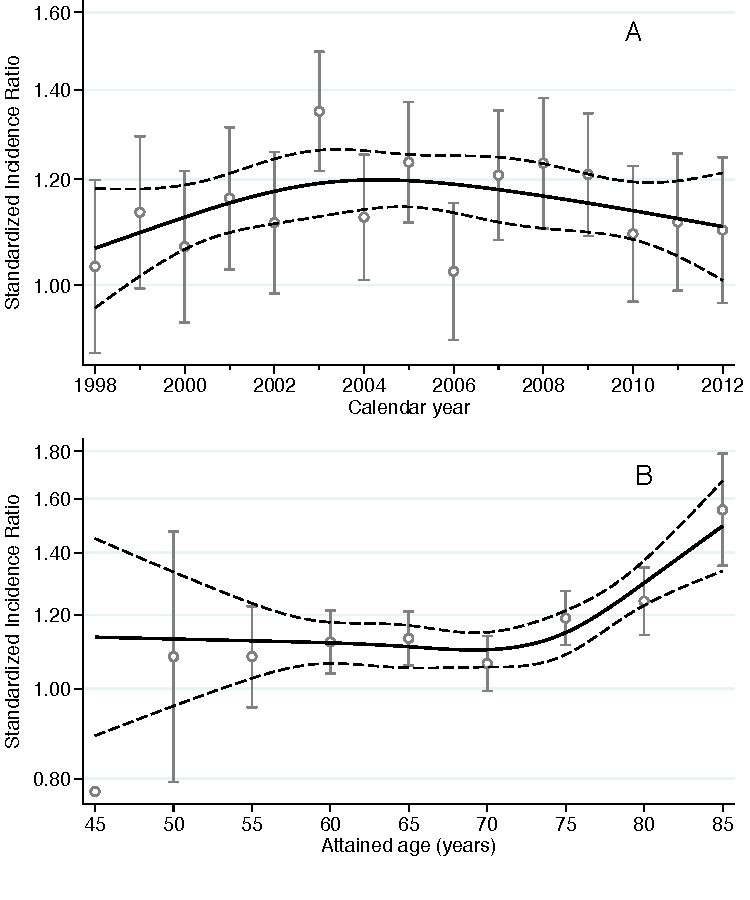
\includegraphics[width=\linewidth]{figures/sir.pdf}
\caption[Standardized Incidence Ratios of prostate cancer by calendar year and attained age]{SIRs of prostate cancer by calendar year (panel A) and attained age (panel B). The solid lines are model-based predicted SIRs, while dashed lines are 95\% confidence intervals. The hollow circles represent the observed SIRs by 5-year groups of attained age and calendar year together with 95\% confidence intervals. The confidence interval for $\SIR_{1,\LargerCdot}$ was not displayed since extremely wide, as it was based on 1 case only (see table \ref{table:appendix_sir_table}). The vertical axes are on the natural log scale.}
\label{fig:sir}
\end{figure}





\subsection{Prostate cancer mortality}

\subsubsection{Prostate cancer mortality in the COSM}

Between 1 January 1998 and 31 December 2012, a total of 691 deaths whose underlying cause was attributed to prostate cancer were observed in the COSM (CDR data). Figure \ref{fig:mr_cosm} shows prostate cancer MRs by attained age and calendar year. The solid lines are the model-based MRs from a `flexible' PH regression model, where attained age was modeled using RCS with 3 knots at 67, 80, and 87 years of age. The PH assumption was once again relaxed via time-dependent coefficients for calendar year. %The hollow circles represent the observed MRs by 5-year categories of attained age and calendar year. 

The interpretation of the analysis on prostate cancer mortality is affected by the fact that the COSM is a cohort of cancer-free men at baseline. In fact, as described previously, all men with a prevalent cancer diagnosis at baseline were excluded from the study. It is therefore not surprising that the prostate cancer MRs were very low during the first years of follow-up, even at older ages. For example, in 1998 only 2 deaths due to prostate cancer were observed. On the other hand, during the last years of follow-up, the mortality curves showed a very steep increase at older ages, in line with what one would expect.

Over the 15 years of follow-up, the MR was shown to be 9\% lower among those men residing in Västmanland county at baseline as compared with those men residing in Örebro county [Mortality Rate Ratio (MRR): 0.91 (95\% CI: 0.78--1.06)]. Similarly, restricting the analysis to the last 6 years of follow-up (2007--2012, 406 prostate cancer deaths), the MRR was observed to be 0.88 (95\% CI: 0.72--1.07). 

The lower prostate cancer--specific mortality\footnote{Prostate cancer--specific mortality refers to mortality due to prostate cancer among men diagnosed with the disease.} observed in Sweden by \citet{stattin_prostate_2014} in high-incidence counties as compared with low-incidence counties, among men aged 50--74 years and during the years 2000--2009 [RR: 0.87 (95\% CI: 0.81--0.95)], was similar to that observed between Västmanland and Örebro counties in the COSM [prostate cancer--specific MRR: 0.85 (95\% CI: 0.73--0.99)].

\begin{sidewaysfigure}
\centering
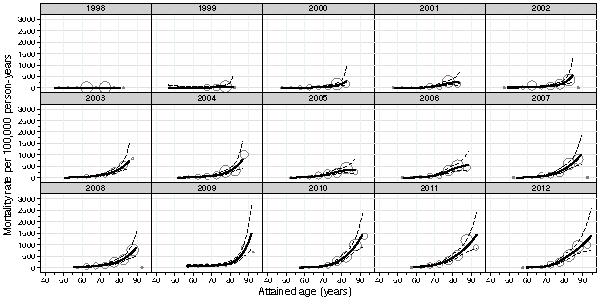
\includegraphics[width=\linewidth]{figures/mr_cosm.pdf}
\caption[Prostate cancer mortality rates in the COSM by calendar year and attained age]{Prostate cancer mortality rates  in the COSM, conditional on calendar year and attained age. The solid line is the model-based predicted incidence rate, while dashed lines are 95\% confidence intervals. Note that the confidence interval for year 1998 is not displayed due to only 2 prostate cancer deaths during the whole year. The hollow circles represent the observed incidence rate by calendar year and 5-year groups of attained age. Their size is proportional to the precision (inverse of the variance) of the estimate. }
\label{fig:mr_cosm}
\end{sidewaysfigure}

\subsubsection{Comparison with Swedish national data}

Comparison of prostate cancer MRs between COSM and Swedish national data was carried out in terms of Standardized Mortality Ratios (SMRs). Source of Swedish data, statistical tools, and notation are identical to those described in section \ref{section:materials_incpca}.

Table \ref{table:appendix_smr_table} reports the number of observed (top entry) and expected (bottom entry) prostate cancer deaths in the COSM according to attained age categories and calendar year. Overall, $\SMR_{\LargerCdot, \LargerCdot} = 691 / 1034  = 0.67$, with 95\% exact CI equal to 0.62--0.72. Again, this is not surprising given that the comparison was made between two populations, one of which was cancer-free at baseline while the other one was not.

Figure \ref{fig:smr_cy} shows the observed SMRs by calendar year calculated marginally over categories of attained age (hollow circles), as well as the SMR modeled as a function of calendar year using RCS with 4 knots positioned at years 1998, 2002, 2007, and 2012 (solid line). In the RCS model, there was evidence of an association between calendar year and SMR ($p_{\textrm{overall}}<0.001$) and also of non-linearity ($p_{\textrm{non-linearity}}<0.001$). The observed SMRs were as low as 0.05 in 1998 [$\SMR_{\LargerCdot, 1998}=2/43=0.05$ (95\% exact CI: 0.01--0.17)], and increased over calendar year to level off after, say, year 2004/2005, not far from the value of 1. %In particular, there was no evidence against the null hypothesis that the SMRs for the last three consecutive years of follow-up (2010--2012) were jointly equal to 1 ($p=0.29$).  
At the same time, no systematic variation in SMR was observed when modeled as a function of attained age (figure \ref{fig:appendix_smr_cage}).

One might have expected a longer time period before the SMRs approached values closer to 1, given the long latency of prostate cancer. However, the COSM was `cancer-free at baseline' only in the sense that those men with a prevalent cancer diagnosis were excluded. Therefore, men with an undiagnosed prostate cancer were still included in the cohort. This can have contributed to a relatively shorter period before the prostate cancer MRs in the COSM reached comparable levels to those observed in Sweden.

Lastly, considering the years 2006--2012 only, there was no evidence that the SMR for those men enrolled in Västmanland county [$\SMR_{\LargerCdot, \textrm{2006--2012}}=210/278 = 0.75$ (95\% exact CI: 0.66--0.86)] was different from that for those men enrolled in Örebro county [$\SMR_{\LargerCdot, \textrm{2006--2012}}=251/289 = 0.87$ (95\% exact CI: 0.76--0.98)] ($p_{\mathrm{heterogeneity}} = 0.14$).


\begin{figure}[hb]
\centering
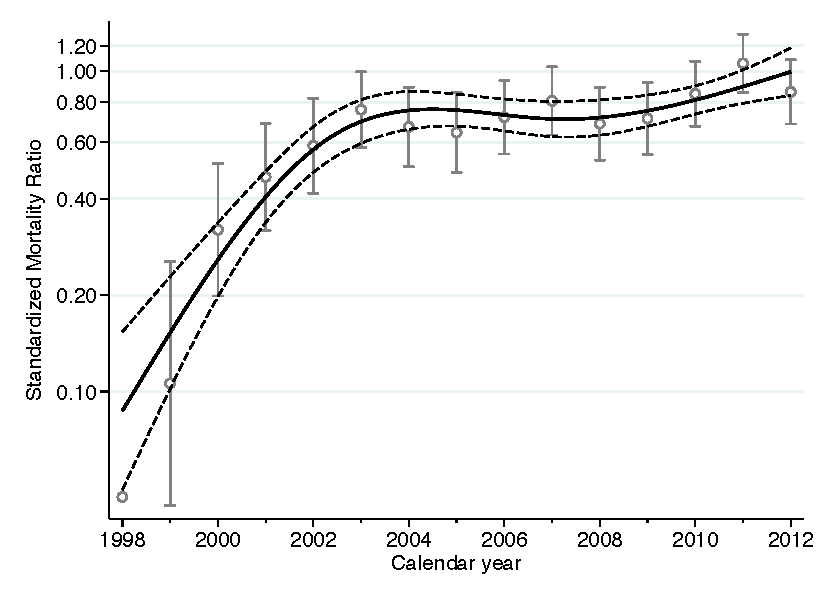
\includegraphics[width=\linewidth]{figures/smr_cy.pdf}
\caption[Standardized Mortality Ratios of prostate cancer by calendar year]{SMRs of prostate cancer by calendar year. The solid line is the model-based predicted SMR, while dashed lines are 95\% confidence intervals. The hollow circles represent the observed SMRs by calendar year together with 95\% confidence intervals. The confidence interval for $\SIR_{\LargerCdot, 1998}$ was not displayed since extremely wide, as it was based on 2 deaths only (table \ref{table:appendix_smr_table}). The vertical axis is on the natural log scale.}
\label{fig:smr_cy}
\end{figure}



